\chapter{Simulation des robots}
\chaptermark{Robots}
\label{chapitre:robots}
	
	\section{Introduction}

		L'environnement dans lequel doivent évoluer les robots à été défini dans le \textsc{Chapitre}~\ref{chapitre:environnement}. Il est maintenant temps de simuler les \gls{ROV}s. Pour ce faire, nous allons devoir décrire les paramètres mécaniques des robots \gls{Argos} et \gls{Atoll}, et décrire le comportement de leurs capteurs et actionneurs à simuler. A la fin de cette partie nous devrions être en mesure de pleinement simuler les robots dans leur environnement, et le simulateur complet devrait ainsi respecter toutes les exigences présentées dans le \textsc{Chapitre}~\ref{chapitre:systeme}.

	\section{Simulation des composants}

		\subsection{Liste des composants}
			En remarquant que les deux robots embarquent un certain nombre d'éléments communs, il est possible de definir et de simuler ces différents composants dans \gls{Gazebo}, afin d'être par la suite chargés dans la simulation des deux robots. La \textsc{table}~\ref{table:components} présente les différents composants à simuler, s'ils nécéssitent l'utilisation d'un \gls{Plugin}, d'une \gls{HardwareInterface} et indique les dépendances entre les robots et ces composants.

		\begin{table}[!htb]
			\centering
			\begin{adjustbox}{max width=\textwidth}
				\begin{tabular}{|l|l|c|c|c|c|}
					\hline
					Composant & Description & \gls{Argos} & \gls{Atoll} & \gls{HardwareInterface} & \gls{Gazebo} \gls{Plugin} \\
					\hline
					\gls{Argos} Frame & Chassis d'\gls{Argos} & \cmark & \xmark & \xmark & \xmark \\
					\hline
					\gls{Atoll} Frame & Chassis d'\gls{Atoll} & \xmark & \cmark & \xmark & \xmark \\
					\hline
					Electronic Pod & Boîtier electronique & \cmark & \cmark & \xmark & \xmark \\
					\hline
					\gls{Latch} & Crochet de levage & \xmark & \cmark & \cmark & \cmark \\
					\hline
					\gls{Navcam} & Caméra de navigation & \cmark & \cmark & \xmark & \cmark \\
					\hline
					\gls{Obscam} & Caméra d'observation & \cmark & \cmark & \xmark & \cmark \\
					\hline
					Rovins & Centrale Inertielle & \cmark & \cmark & \xmark & \cmark \\
					\hline
					Spotlight & Lumières étanches & \cmark & \cmark  & \cmark & \cmark \\
					\hline
					SPE75 Thruster & Propulseur & \cmark & \cmark & \cmark & \cmark \\
					\hline
					SS309 Tilt & Nacelle pour caméra & \cmark & \cmark & \cmark & \cmark \\
					\hline
				\end{tabular}}
			\end{adjustbox}
			\caption{Composants à simuler}
			\label{table:components}
		\end{table}

		\subsection{Séparation Packages}

			La convention \gls{ROS2} et \gls{Gazebo} pour la description des robots dans le but de les simuler prévoit de répartir le code dans différents paquets. Nous allons appliquer ici cette même convention pour chaque composant à simuler.

			\begin{itemize}
				\renewcommand{\labelitemi}{\textbullet}
				\item \textit{composant\_description} :
				\begin{itemize}[noitemsep]
					\item Description URDF comportant les couches visuelles, inertielles et de collision
					\item Maillages 3D permettant de représenter visuellement le composant
					\item Fichier de configuration pour visualiser le composant dans RViz2
				\end{itemize}
				\item \textit{composant\_gazebo} :
				\begin{itemize}[noitemsep]
					\item \gls{Plugin} décrivant le comportement du composant dans \gls{Gazebo}
					\item Ficher de lancement du composant dans \gls{Gazebo}
				\end{itemize}
			\end{itemize}

		Nous allons à présent détailler l'implémentation de certains composants qui ont un comportement intéressant à développer.

		\subsection{Latch}

			\subsubsection{Présentation}

				Le Latch est un composant propre au robot \gls{Atoll}. Ce crochet de levage permettant de transporter des structures sous-marines pouvant peser jusqu'à $1,5\ T$ est fabriqué par Forssea Robotics, et permet de positionner et de transporter des balises de positionnement acoustique sur les fonds marins.

			\subsubsection{Hardware Interface}


				
			\subsubsection{Model Plugin}
			
				Un \textit{Model Plugin} a été développé afin de décrire le comportement du \textit{Latch} dans \gls{Gazebo}. Il est basé sur la machine à états finis présenté en \textsc{Figure}~\ref{fig:latch_fsm} et crée un \gls{Joint} entre le \textit{Latch} et la structure à soulever de type encastrement. Les deux solides sont donc attachés l'un à l'autre jusqu'au moment où le signal de relâchement est envoyé au \textit{Latch} simulé, et le \gls{Joint} est alors supprimé.

				\begin{figure}[!htb]
					\centering
					\includegraphics[scale=0.8]{imgs/latch_fsm.pdf}
					\caption{Machine à états du \textit{Latch}}
					\label{fig:latch_fsm}
				\end{figure}

			\subsubsection{Résultats}

				On obtient alors le composant simulable dans l'environnement de simulation \gls{Gazebo}, comme on peut voir sur la \textsc{Figure}~\ref{fig:latch_gazebo}.

		\subsection{SS309 Tilt}

			\subsubsection{Présentation}

				Le \textit{SS309 Tilt} est un composant commercialisé par l'entreprise \textit{Sidus Solutions} et qui permet dans les \gls{ROV}s d'orienter l'\gls{Obscam}. Il est parfaitement étanche et comporte un jeu d'engrenages reliés à un moteur pas-à-pas pilotable en vitesse et en position. On demande ainsi au moteur de mettre l'axe à une certaine position, et l'axe se déplace avec une vitesse de rotation spécifiée.
			
			\subsubsection{Hardware Interface}

			\subsubsection{Model Plugin}

				Pour simuler cet aspect pilotable en vitesse de rotation et position, il faut passer par la simulation d'un moteur pas-à-pas. C'est un moteur un moteur composé de plusieurs bobinages créant ainsi plusieurs phases qui sont allumées succéssivement afin de réaliser une rotation de l'arbre moteur d'un certain incrément d'angle. Cet angle est défini par les caractéristiques du bobinage et n'est donc pas réglable. Il n'est pas non plus possible de piloter précisement la vitesse avec laquelle il se rend à cette position incrémentée. En revanche, il est tout à fait possible de connaître précisement la position du moteur, car l'arbre moteur ne peut prendre qu'un nombre fini d'angles, et il suffit donc de compter le nombre d'incréments commandés. Enfin, on peut commander la vitesse avec laquelle le moteur se rend à cette position, en allumant les phases à la vitesse désirée.

				Nous allons à présent distinguer la position réelle de l'arbre moteur, la position cible et la position commandée. La position réelle est la position de l'arbre moteur dans le simulateur. La position cible est un multiple de l'incrément d'angle à laquelle doit se rendre le moteur à l'instant actuel. La position commandée la position finale dans laquelle doit se retrouver l'arbre moteur et peut être une position réelle quelconque. Le moteur ne sera capable que de se rendre à la position multiple de la valeur de l'incrément d'angle la plus proche de la position commandée. La \textsc{Figure}~\ref{fig:tilt_position} reprends ces différentes notions. En commandant la vitesse à laquelle on incrémente la position cible, on contrôle l'axe en vitesse.

				\begin{figure}[!htb]
					\centering
					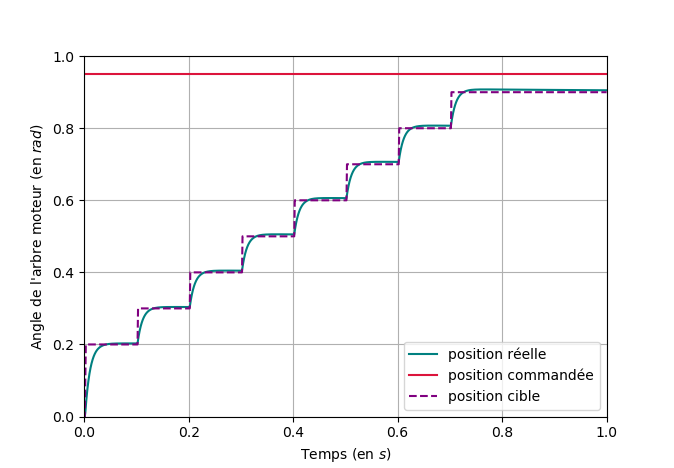
\includegraphics[width=0.6\textwidth]{imgs/stepper_motor.png}
					\caption{Simulation d'un moteur pas-à-pas}
					\label{fig:tilt_position}
				\end{figure}
				
				Pour ce qui est de l'implémentation de ce comportement dans \gls{Gazebo}, on crée un \textit{Thread} qui va s'executer en boucle avec une vitesse variable. Cette vitesse sera fonction de la vitesse de commande du \textit{Tilt} notée $\omega_c$. A chaque tour de boucle, on incrémente donc la position cible de la valeur de l'incrément $d\theta$ si la différence entre la position réelle et la position commandée est plus grande que ce même incrément, et on attends le temps $h$, avec :

				$$h = \frac{d\theta}{\omega_c}$$

				\begin{algorithm}[!htb]
					\caption{Algorithme de simulation d'un moteur pas-à-pas}
					\label{algo:stepper_motor}
					\begin{algorithmic}
						\WHILE {true}
							\STATE read $\theta_r$, $\omega_c$
							\IF {$|\theta_c - \theta_r| > d\theta$}
								\STATE $\theta_t \leftarrow \theta_t + d\theta$
							\ENDIF
							\STATE $h \leftarrow \frac{d\theta}{\omega_c}$
							\STATE sleep $h$
						\ENDWHILE
					\end{algorithmic}
				\end{algorithm}

		\subsection{SPE75 Thrusters}

			\subsubsection{Présentation}
	
				Les \textit{SPE75 Thrusters} sont les propulseurs qui permettent aux robots de se déplacer et de s'orienter dans leur environnements. Ils sont composés d'un moteur permettant de mettre en mouvement des pale qui va permettre de générer une force dans la direction du propulseur.
				
			\subsubsection{Hardware Interface}

				L'\textit{Hardware Interface} va proposer une interface aux contrôleurs permettant d'appliquer une force suivant l'axe du propulseur qui va être transmise au robot. Elle va ensuite se charger de calculer la vitesse de rotation des pales nécéssaire à la création de cette force. Pour le composant réel, cette vitesse va être transmise au propulseur qui générer la force voulue et un couple résistant dans le sens inverse de la rotation des pâles sur le corps du propulseur qui va être transmis au robot. Pour le composant simulé, on est en mesure d'intéragir avec le simulateur afin d'appliquer des forces et des couples directement sur les objets simulés. 
				
				Le calcul de la vitesse de rotation des pâles en fonction de la force demandée est réalisé grâce à une interpolation de points de mesures faits sur un banc d'essai. L'idée est de faire tourner en eau le propulseur fixé sur un capteur de force à une certaine vitesse, et de mesurer la force générée par celui-ci. Ensuite, on est capable d'interpoler les pointsexpérimentaux logiciellement à l'aide de la librairie \gls{GSL}\footnote{\url{https://www.gnu.org/software/gsl/}} et de la fonctionnalité \textit{spline}. On peut ainsi calculer une vitesse de rotation à appliquer quel que soit la valeur de force demandée.
				
				L'idée retenue pour ce simulateur est d'appliquer directement la force demandée sur le corps du propulseur, car il est assez difficile et coûteux en ressources de calculs de realiser de la mécanique des fluides afin de simuler pleinement le comportement des pâles du propulseur. Il est tout de même nécéssaire de faire tourner les pâles dans le simulateur, car outre l'aspect cosmétique de voir les pales tourner quand le moteur fournit une poussée au robot, le simple fait de faire tourner ce solide ayant une certaine masse dans le simulateur va générer le couple résistant sur le corps du propulseur. Ainsi cette \textit{Hardware Interface} va communiquer au \textit{Model Plugin} la force et la vitesse de rotation des pâles calculée à appliquer sur le propulseur simulé.
	
			\subsubsection{Model Plugin}

				Le \textit{Model Plugin} va se charger d'appliquer la force et la vitesse de rotation communiquée par l'\textit{Hardware Interface}. Le \textit{plugin} est chargé pour chaque propulseur simulé et permet d'accéder finement aux paramètres de la simulation. On peut alors appliquer à chaque incrément de simulation la force demandée sur le corps du propulseur et la vitesse de rotation sur la liaison pivot entre le corps du propulseur et les pâles.
				

	\section{Simulation d'Argos}

	\section{Simulation d'Atoll}

	\section{Conclusion}